\chapter{شناسایی جت‌های بوست‌شده با شبکه‌های عصبی گرافی کوانتومی مبتنی بر هامیلتونی}
\label{ch:tagger}

\section*{چکیده}
یک شناساگر ترکیبی کوانتومی و کلاسیک برای شناسایی جت‌هایی با بوست لورنتس بزرگ در برخورددهنده‌ها ارائه می‌کنیم که در آن داده‌های گرافی جت به‌صورت یک بازنمایی گرافی کوانتومی رمزگذاری می‌شوند و با یک شبکه عصبی گرافی کوانتومی وردشی (\lr{QGNN}) طبقه‌بندی می‌شوند. مدل برای تمایز جت‌های حاصل از واپاشی هادرونی بوزون \Zbos{} بوست‌شده از جت‌های گلوئونی پرتکانه طراحی شده است. برای امکان اجرا روی سخت‌افزار کوانتومی نزدیک‌آینده، اطلاعات پُربعد جت با یک رمزگذار کلاسیک که هم‌زمان بهینه می‌شود و منظم‌سازی توزیعی مبتنی بر سینخورن دارد به یک بازنمایی گرافی نهان کم‌بعد فشرده می‌شود. بازنمایی‌های نهان سپس به‌صورت داده گرافی رمزگذاری می‌شوند و با یک \lr{QGNN} ده‌کیوبیتی مبتنی بر هامیلتونی پردازش می‌شوند، و رمزگذار و جداکننده کوانتومی در یک آموزش سرتاسری با هم بهینه می‌شوند. مدل ترکیبی حاصل عملکردی قابل‌مقایسه با یک شبکه عصبی عمیق کلاسیک دارد و به عملکرد یک جداکننده گرافی در سطح دانش روز نزدیک می‌شود. تا آنجا که می‌دانیم این نخستین شناساگر جت بوست‌شده است که اطلاعات جت را در یک بازنمایی گرافی کوانتومی رمزگذاری می‌کند تا یک شبکه عصبی گرافی کوانتومی آن را پردازش کند.

\begin{figure}[H]
\centering
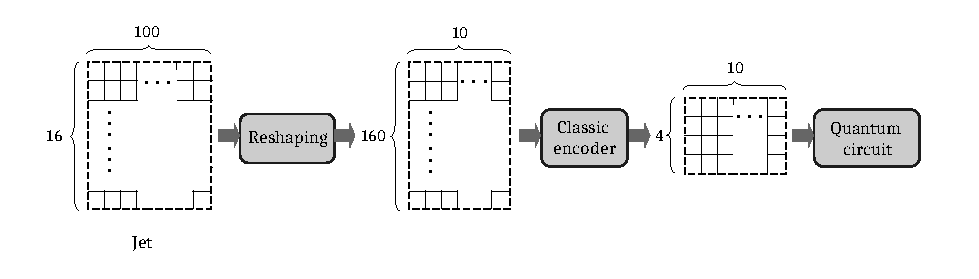
\includegraphics[width=\textwidth]{ch1_overview}
\caption{نمای کلی فرایند شناسایی: جت پس از بازشکل‌دهی به یک آرایه $10\times160$ از طریق لایه‌های کلاسیک به ابعاد $10\times4$ تبدیل می‌شود و سپس در یک مدار کوانتومی با پارامترهای قابل آموزش رمزگذاری می‌شود. لایه‌های کلاسیک و کوانتومی با هم آموزش داده می‌شوند تا سیگنال از پس‌زمینه جدا شود.}
\label{fig:ch1-overview}
\end{figure}

\section{داده‌های شبیه‌سازی‌شده و پیش‌پردازش}
\label{sec:ch1-data}
از نمونه‌ای شامل ۲۰۰۰۰ جت شبیه‌سازی‌شده با تکانه بالا استفاده می‌شود که به‌طور مساوی بین دو دسته، جت‌های ناشی از بوزون \Zbos{} و جت‌های ناشی از گلوئون، تقسیم شده است~\cite{Pierini:JetDataset}. جت‌ها به‌طور میانگین ۱۰۰ ذره دارند و هر ذره با ۱۶ ویژگی توصیف می‌شود. از هر ذره $i$ سه مؤلفه بردار تکانه $\vec p_i$، انرژی $E_i$ و تکانه عرضی $p_{\mathrm{T},i}$ همراه با نسبت آنها به مقدار متناظر جت در نظر گرفته می‌شود. افزون بر این، مختصات هر ذره در شبه‌سرعت $\eta_i$ و زاویه سمتی $\varphi_i$، اختلاف آنها با مختصات متناظر جت، مقدارشان در یک دستگاه مختصات چرخیده، و نیز فاصله آنها از محور جت در صفحه $(\eta,\varphi)$، یعنی $\Delta R=\sqrt{\Delta\varphi_i^2+\Delta\eta_i^2}$، از جمله ویژگی‌های دیگر مورد استفاده‌اند. در پایان، کسینوس زاویه پراکندگی ذره را نسبت به محور برخورد و نسبت به محور جت به‌عنوان ویژگی‌های اضافی برمی‌داریم. با این ۱۶ ویژگی برای هر ذره، هر جت در تحلیل به‌صورت یک آرایه با اندازه $100\times16$ نمایش داده می‌شود.

در مرحله پیش‌پردازش، ده ذره اول را بر حسب $E$ در هر جت انتخاب می‌کنیم و بردار ویژگی آنها را با $\{\mathbf{x}_1,\dots,\mathbf{x}_{10}\}\in\mathbb{R}^{16}$ نشان می‌دهیم. برای هر ذره انتخاب‌شده $i\in\{1,\dots,10\}$، ده نزدیک‌ترین همسایه را در میان همه ذره‌های $k$ موجود در جت بر حسب $\Delta R(i,k)$ پیدا و مرتب می‌کنیم. سپس قدر مطلق اختلاف بردارهای ویژگی، $\boldsymbol{\delta}_{ik}\equiv|\mathbf{x}_i-\mathbf{x}_k|\in\mathbb{R}^{16}$، برای $k$ که روی نزدیک‌ترین همسایه‌ها می‌گذرد محاسبه می‌شود. با الحاق $\boldsymbol{\delta}_{ik}$ روی اندیس $k$ یک بردار ویژگی جدید با بعد ۱۶۰ برای هر ذره $i$ به دست می‌آید. به این ترتیب هر جت به آرایه‌ای از ده ذره با ۱۶۰ ویژگی تبدیل می‌شود، یعنی $\mathbf{X}^{(j)}\in\mathbb{R}^{10\times160}$، که توپولوژی محلی و اطلاعات سینماتیکی را در قالبی سازگار با گراف رمزگذاری می‌کند. این ساختار نسبت به جابه‌جایی هر جفت از ذره‌های همسایه اولیه، یعنی $i\leftrightarrow k$ در $\boldsymbol{\delta}_{ik}$، ناورداست.

جت‌های پیش‌پردازش‌شده از طریق رمزگذار کلاسیک به داده‌های $\mathbf{X}^{(j)}\in\mathbb{R}^{10\times4}$ تبدیل می‌شوند و سپس با مدار کوانتومی طبقه‌بندی می‌شوند. هر دو بخش کلاسیک و کوانتومی پارامترهای قابل آموزش دارند و در نهایت با هم آموزش داده می‌شوند.

\section{رمزگذار کلاسیک}
\label{sec:ch1-encoder}
بازنمایی‌های پُربعد جت در آزمایش‌های برخورددهنده برای فرایندهای طبقه‌بندی تقویت‌شده با کوانتوم چالش‌های جدی ایجاد می‌کنند، به‌ویژه به‌دلیل محدودیت تعداد کیوبیت‌ها، نویز دروازه‌ها و عمق کم مدارها در دستگاه‌های \lr{NISQ}~\cite{Odagiu:2025,Belis:2024}. بنابراین گام بعدی ساختن یک بازنمایی نهان (\lr{latent}) است که برای پردازش کوانتومی به‌اندازه کافی فشرده باشد و در عین حال اطلاعات مربوط به تمایز جت‌ها را نگه دارد. خودرمزگذارهای بهینه‌شده به‌طور گسترده برای کاهش مؤثر بعد به کار می‌روند، به‌گونه‌ای که اطلاعات زیرساختار جت لازم برای تمایز را حفظ می‌کنند و در عین حال سازگاری با مدارهای کوانتومی را ممکن می‌سازند.

در شناساگر ما، کاهش بعد با بخش رمزگذار یک خودرمزگذار انجام می‌شود که عملکرد آن به تفصیل بررسی شده است. با الهام از مرجع~\cite{Kamil:2020}، از یک خودرمزگذار سینخورن سرتاسری برای فشرده‌سازی داده‌ها استفاده می‌کنیم تا جداپذیری دسته‌ها حفظ شود و ناهم‌خوانی توزیع کلاسیک به کوانتومی کاهش یابد. برخلاف خودرمزگذارهای سینخورن معمول، فضای نهان رمزگذاری‌شده از طریق واگرایی سینخورن به سمت یک توزیع نهان مرجع آموخته‌شده منظم‌سازی می‌شود و این امکان را می‌دهد که منظم‌سازی توزیعی تطبیقی در طول آموزش مشترک انجام شود. به‌عنوان معیار مقایسه، داده‌های جت با تحلیل مؤلفه‌های اصلی (\lr{PCA})~\cite{Pearson:1901} هم فشرده می‌شوند. داده‌های فضاهای نهان \lr{PCA} و خودرمزگذار سپس به الگوریتم \lr{ParticleNet} داده می‌شوند و عملکرد تمایز جت‌ها مقایسه می‌شود. تنظیمات الگوریتم \lr{ParticleNet} از مرجع~\cite{Qu:2019gqs} پیروی می‌کند که در آن تعداد نزدیک‌ترین همسایه‌ها به‌طور خاص ۷ است. داده‌ها، که شامل تعداد مساوی جت \Zbos{} و جت گلوئونی‌اند، به نمونه آموزش با ۱۰۰۰۰ جت و نمونه‌های اعتبارسنجی و آزمون هر کدام با ۵۰۰۰ جت تقسیم می‌شوند. بردارهای ویژگی ۱۶۰‌بعدی طوری بهنجار می‌شوند که مقادیر بین ۰ و ۱ باشند و بهنجارش روی نمونه آموزش برازش می‌شود.

خودرمزگذار پایه داده‌ها را با سه لایه تبدیل خطی ($160\to128\to64\to4$) و توابع فعال‌سازی یکسوساز خطی (\lr{ReLU})~\cite{Glorot:2011,Maas:2013} میان آنها رمزگذاری می‌کند. داده‌ها با ساختاری وارون رمزگشایی می‌شوند و با ورودی مقایسه می‌شوند و تابع زیان میانگین مربعات خطا (\lr{MSE}) است. یک نمونه مصنوعی با ۶۴ ویژگی با نمونه‌برداری مستقل هر ویژگی از توزیع یکنواخت روی $[0,1]$ تولید می‌شود. به نمونه‌های مصنوعی به‌طور تصادفی برچسب سیگنال یا پس‌زمینه داده می‌شود و از یک مولد قابل آموزش عبور داده می‌شوند که از لایه‌های خطی تشکیل شده است و بعد ویژگی را از ۶۴ به ۱۲۸ افزایش می‌دهد و سپس با توابع فعال‌سازی \lr{ReLU} آن را به چهار بُعد فشرده می‌کند. بردارهای نهان حاصل به آرایه‌های $10\times4$ بازشکل داده می‌شوند و یک بازنمایی نهان مرجع آموخته‌شده را می‌سازند که منحصراً برای منظم‌سازی سینخورن به کار می‌رود. در آموزش، یک واگرایی سینخورن بدون سوگیری (\lr{debiased}) بازنمایی‌های نهان تولیدشده با رمزگذار کلاسیک را با توزیع نهان مرجع آموخته‌شده هم‌تراز می‌کند؛ این کار از طریق تطبیق انتقال بهینه آگاه از برچسب انجام می‌شود و تضمین می‌کند که نمونه‌های سیگنال و پس‌زمینه به توزیع‌های مرجع متناظر خود منتقل شوند. برخلاف منظم‌سازی نهان معمول مبتنی بر یک پیشین ثابت، توزیع مرجع هم‌زمان با رمزگذار آموخته می‌شود و منظم‌سازی توزیعی تطبیقی فراهم می‌کند که استواری و قدرت تعمیم بازنمایی نهان را بهبود می‌دهد. برای خودرمزگذار سینخورن سرتاسری، تابع زیان مجموع وزن‌دار \lr{MSE} پایه و واگرایی سینخورن بدون سوگیری~\cite{Cuturi:2013} است که سهم نسبی دومی \lr{0.001} است. مدل، که در مجموع $6\times10^{4}$ پارامتر دارد، با بهینه‌ساز \lr{Adam}~\cite{Kingma:2014} بهینه می‌شود و ۲۰ دوره با اندازه دسته ۱۶ و نرخ یادگیری \lr{0.0001} آموزش می‌بیند.

عملکرد الگوریتم \lr{ParticleNet} روی داده‌های فشرده‌شده معیار و روی فضاهای نهان خودرمزگذارهای پایه و سینخورن ارزیابی شده و در شکل~\ref{fig:ch1-pn} خلاصه شده است. سه روش در محدوده عدم‌قطعیت‌ها نتایج قابل‌مقایسه‌ای می‌دهند. این مشاهده استفاده از بازنمایی نهان آموخته‌شده را در بخش بعد توجیه می‌کند، که در آن بازنمایی به گراف تبدیل و با \lr{QGNN} پردازش می‌شود. رمزگذار نهایی بر پایه آموزش مشترک سرتاسری با \lr{QGNN} انتخاب می‌شود و \lr{PCA} کنار گذاشته می‌شود، چون برای بهینه‌سازی مشترک مناسب نیست.

\begin{figure}[H]
\centering
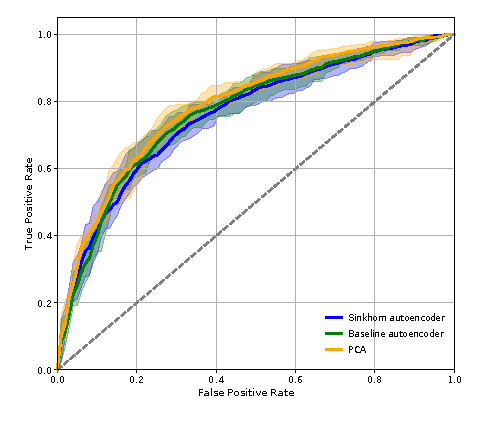
\includegraphics[width=0.6\textwidth]{ch1_roc_latent}
\caption{عملکرد مستقل \lr{ParticleNet} روی بازنمایی‌های نهان $10\times4$ حاصل از روش‌های مختلف فشرده‌سازی، به‌صورتی که در متن توضیح داده شد. نوارهای سایه‌دار بازه $\pm1\sigma$ حاصل از اعتبارسنجی متقاطع پنج‌گانه را نشان می‌دهند.}
\label{fig:ch1-pn}
\end{figure}

\section{داده‌های گرافی و مدار کوانتومی}
\label{sec:ch1-qgnn}
داده‌های فضای نهان با بعد $10\times4$ روی گرافی با ده گره نگاشت می‌شوند که هر گره چهار ویژگی دارد. هر گره به سه نزدیک‌ترین همسایه خود بر حسب فاصله اقلیدسی در فضای ویژگی چهاربعدی متصل می‌شود. ویژگی‌های یال به‌صورت فاصله بین دو گره متصل تعریف می‌شوند. داده‌های گراف به یک شبکه عصبی گرافی کوانتومی مبتنی بر هامیلتونی داده می‌شوند تا جت‌های \Zbos{} را از جت‌های گلوئونی تمایز دهد. مدار کوانتومی ده‌کیوبیتی با چارچوب \lr{PennyLane}~\cite{Bergholm:2018} شبیه‌سازی می‌شود و گرادیان‌ها با روش مشتق‌گیری الحاقی (\lr{adjoint differentiation})~\cite{Jones:2020} محاسبه می‌شوند. مدار را می‌توان به‌صورت چهار مرحله متوالی دید، مطابق شکل~\ref{fig:ch1-circuit}. در بخش اول، ویژگی‌های گره با روش بارگذاری مجدد داده (\lr{data re-uploading})~\cite{PerezSalinas:2019} وارد می‌شوند. بخش دوم شامل یک عملگر تحول زمانی یکانی است که هامیلتونی در آن اطلاعات مجاورت (ویژگی‌های یال) گراف را رمزگذاری می‌کند. این عملگر با بسط مرتبه اول تروتر-سوزوکی و با یک گام تروتر در هر لایه~\cite{Trotter:1959} تقریب زده می‌شود و زمان تحول به‌عنوان یک پارامتر قابل آموزش در نظر گرفته می‌شود. در بخش سوم یک مدار کوانتومی وردشی (\lr{VQC}) برای فراگیری اطلاعات سراسری گراف طراحی شده است. خروجی مدار در بخش آخر با اندازه‌گیری روی همه کیوبیت‌ها تعیین می‌شود. چند معماری مدار کوانتومی، به‌ویژه برای مرحله بارگذاری ویژگی‌ها، بررسی شده است تا طرح مؤثر پیدا شود. برای اینکه جست‌وجوی معماری از نظر محاسباتی ممکن بماند، از نمونه کاهش‌یافته‌ای از ۸۰۰۰ جت استفاده می‌شود که ۴۰۰۰ جت آن برای آموزش، ۲۰۰۰ برای اعتبارسنجی و ۲۰۰۰ برای آزمون است. مدل، با ۲۸۱ پارامتر قابل آموزش، با بهینه‌ساز \lr{Adam} با نرخ یادگیری اولیه \lr{0.005} و تضعیف وزن $10^{-4}$ آموزش داده می‌شود. وقتی زیان اعتبارسنجی پنج دوره ثابت بماند نرخ یادگیری نصف می‌شود. اندازه دسته ۲ و ده دوره برای آموزش کافی تشخیص داده شد.

\begin{figure}[H]
\centering
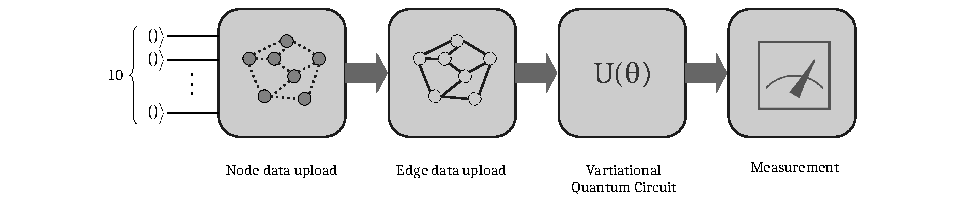
\includegraphics[width=\textwidth]{ch1_circuit}
\caption{ساختار کلی مدار کوانتومی که چهار بخش دارد: بارگذاری مجدد ویژگی‌های گره، تحول هامیلتونی برای رمزگذاری یال‌ها، مدار وردشی \lr{VQC} برای یادگیری گراف به‌صورت یک کل، و خروجی اندازه‌گیری.}
\label{fig:ch1-circuit}
\end{figure}

در بخش اول مدار، داده‌های گراف روی مجموعه‌ای از ده کیوبیت $|0\rangle^{\otimes10}$ با ساختاری که در شکل~\ref{fig:ch1-reupload} نشان داده شده بارگذاری می‌شوند. چون گراف ده گره با چهار ویژگی دارد، $\mathbf{x}_g\in\mathbb{R}^{10\times4}$، برای واردکردن همه اطلاعات به مدار به بارگذاری مجدد داده نیاز است، که حالت اولیه کیوبیت‌ها را به
\begin{equation}
|\Psi\rangle=\prod_{k=1}^{4}V_kU_k|0\rangle^{\otimes10},
\end{equation}
با
\begin{equation}
U_k=\bigotimes_{i=1}^{10}R_X(\theta_{ik}),
\end{equation}
تغییر می‌دهد و برای رمزگذاری داده با چرخش حول محور $x$ به کار می‌رود. در اینجا مقدار ویژگی $k$-ام از گره $i$-ام به $[0,2\pi]$ نگاشته می‌شود و با $\theta_{ik}$ نشان داده می‌شود. بلوک‌های رمزگذاری با بلوک‌های وردشی
\begin{equation}
V_k=C_k\bigotimes_{i=1}^{10}R_Z(\gamma_{ik})R_Y(\beta_{ik}),
\end{equation}
درهم‌تنیده‌اند که شامل چرخش‌هایی حول محورهای $y$ و $z$ است و پس از آن دروازه‌های کنترلی $C_k$ می‌آیند. پارامترهای $\gamma_{ik}$ و $\beta_{ik}$ قابل آموزش‌اند. برای $C_k$ سه معماری آزموده شده است: یک زنجیره از دروازه‌های کنترل‌نات (\lr{CNOT})، یعنی $\prod_{i=1}^{9}\mathrm{CNOT}_{i,i+1}$، و یک زنجیره از چرخش‌های کنترل‌شده حول محور $x$ یا $z$ که در آن دروازه‌ها بین هر جفت کیوبیت مجاور قرار می‌گیرند و زاویه‌های چرخش پارامترهای قابل آموزش‌اند. شکل~\ref{fig:ch1-ck} پیاده‌سازی‌های مختلف دروازه‌های کنترلی را نشان می‌دهد. مشاهده کردیم که به‌کارگیری چرخش‌های کنترل‌شده به‌جای \lr{CNOT} استواری و عملکرد را اندکی بهبود می‌دهد.

\begin{figure}[H]
\centering
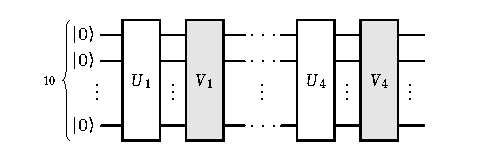
\includegraphics[width=0.55\textwidth]{ch1_reupload}
\caption{مدار کلی بارگذاری مجدد داده با بلوک‌های رمزگذاری $U_k$ و بلوک‌های وردشی $V_k$ که به‌طور متناوب چهار بار روی مدار ده‌کیوبیتی تکرار می‌شوند.}
\label{fig:ch1-reupload}
\end{figure}

\begin{figure}[H]
\centering
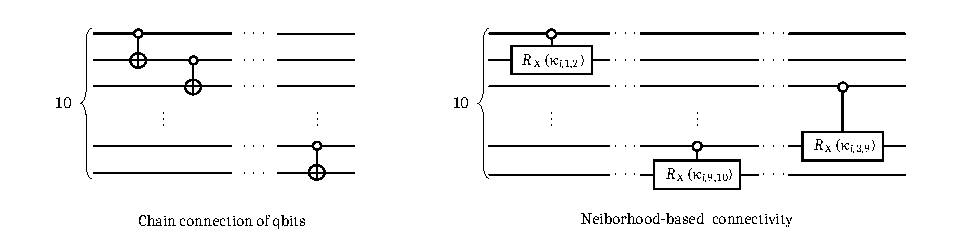
\includegraphics[width=\textwidth]{ch1_ck}
\caption{سه معماری برای $C_k$: زنجیره \lr{CNOT} (چپ) و \lr{CRX} (راست)، هر دو با اتصال میان همسایه‌های مجاور. ساختار \lr{CRZ} مشابه چرخش کنترل‌شده حول محور $x$ است.}
\label{fig:ch1-ck}
\end{figure}

رمزگذاری ویژگی‌های یال از طریق یک تحول هامیلتونی انجام می‌شود که به‌صورت
\begin{equation}
\hat H=\sum_{i<j}\ \sum_{j\in\mathcal{N}_i} w_{ij}\,\hat\sigma_i^{a}\hat\sigma_j^{a},
\end{equation}
تعریف می‌شود. در اینجا برای هر گره $i$، اندیس $j$ روی نزدیک‌ترین همسایه‌های آن، $\mathcal{N}_i$، می‌گذرد. عملگر $\hat\sigma^{a}$ در آزمایش‌های ما ماتریس پائولی برای $a=x$ یا $z$ است و قدرت برهمکنش $w_{ij}$ وارون ویژگی یال متناظر است. $w_{ij}$ در هر گذر رو به جلو متناسب با به‌روزرسانی ویژگی‌های گره تغییر می‌کند. عملکرد وابستگی شدیدی به انتخاب $a$ به‌تنهایی نشان نمی‌دهد؛ بلکه در ترکیب با ساختار بارگذاری مجدد اهمیت می‌یابد، که در آن چرخش‌های کنترل‌شده حول محور $z$ همراه با $\hat\sigma^{x}$ در هامیلتونی بهترین عملکرد را می‌دهند. لایه سوم یک \lr{VQC} است که گراف ورودی را می‌آموزد و اطلاعات گره و یال را ترکیب می‌کند. این لایه از چرخش‌هایی حول محور $y$ روی همه کیوبیت‌ها، $\bigotimes_{i=1}^{10}R_Y(\kappa_i)$، تشکیل شده است که $\kappa_i$ پارامترهای قابل آموزش‌اند. در بخش اندازه‌گیری، مقدار چشم‌داشتی اسپین هر کیوبیت در راستای محور $z$ اندازه‌گیری و روی همه کیوبیت‌ها میانگین‌گیری می‌شود. خروجی $\bar s\in[-1,1]$ با تبدیل آفین $\tfrac{1}{2}(\bar s+1)$ به یک احتمال تبدیل می‌شود و در تابع زیان آنتروپی متقاطع دودویی~\cite{Ramos:2018} برای آموزش مدل به کار می‌رود. اندازه‌گیری خروجی عمداً ساده انتخاب شده است و برای محاسبه صریح همبستگی‌های چندکیوبیتی مرتبه بالا طراحی نشده است. در عوض، حالت کوانتومی حاصل از بخش‌های درهم‌تنیده‌ساز مدار را در یک عدد واحد خلاصه می‌کند. عملکرد مدل وابستگی شدیدی به جهت اندازه‌گیری اسپین نشان نمی‌دهد.

برای سنجش عملکرد، \lr{QGNN} و الگوریتم \lr{ParticleNet} روی داده‌های فضای نهان آموزش داده می‌شوند و مقدار سطح زیر منحنی مشخصه عملکرد گیرنده (\lr{ROC}) یا \lr{AUC} ارزیابی می‌شود. برای مقایسه منصفانه، تعداد نزدیک‌ترین همسایه‌ها در الگوریتم \lr{ParticleNet} برابر ۳ گذاشته می‌شود. مدل ترکیبی \lr{AUC} برابر $0.683\pm0.013$ می‌دهد، در مقایسه با $0.738\pm0.024$ از \lr{ParticleNet}. آموزش هم‌زمان رمزگذار و \lr{QGNN} می‌تواند عملکرد را بهبود دهد، چون آموزش بخش کلاسیک نسبت به تمایز نهایی جت‌ها بی‌اطلاع نیست.

\section{آموزش هم‌زمان}
\label{sec:ch1-joint}
در این بخش آموزش هم‌زمان سرتاسریی رمزگذار کلاسیک و \lr{QGNN} را بررسی می‌کنیم. این مرحله اوج جریان کار است، که در آن بازنمایی نهان و جداکننده کوانتومی با هم بهینه می‌شوند و نه به‌صورت اجزای جداگانه. مدل روی نمونه کامل داده آموزش می‌بیند، که در آن تقسیم داده و اندازه دسته مانند بخش~\ref{sec:ch1-encoder} است و تنظیمات یادگیری مانند بخش~\ref{sec:ch1-qgnn} است، به‌جز تعداد دوره‌ها که ۷۰ است.

داده‌های پیش‌پردازش‌شده، یعنی جت‌هایی با بعد $10\times160$، از رمزگذار عبور می‌کنند و یک بازنمایی نهان ($10\times4$) تولید می‌شود که هم‌زمان با آموزش در اختیار مدار کوانتومی قرار می‌گیرد. برای سنجش اثر مولد نهان قابل آموزش، آموزش با نویز اضافه‌شده و بدون آن انجام می‌شود. آموزش هم‌زمان نسبت به حالت مستقل بیش از ۲۰ درصد بهبود می‌دهد و \lr{AUC} برابر $0.825\pm0.019$ به دست می‌آید. وقتی با روش سینخورن یک فضای نهان احتمالاتی ساخته می‌شود، \lr{AUC} برابر $0.842\pm0.007$ می‌شود که عدم‌قطعیت کوچک‌تری دارد. این رفتار با نقش واگرایی سینخورن به‌عنوان منظم‌ساز توزیعی سازگار است، که هندسه فضای نهان را مقید می‌کند و در نتیجه پایداری و قدرت تعمیم بازنمایی آموخته‌شده را بهبود می‌دهد.

به‌عنوان معیار کلاسیک، \lr{ParticleNet} روی همان داده‌ها با بعد $10\times160$ آموزش داده می‌شود و \lr{AUC} برابر $0.875\pm0.006$ به دست می‌آید. شایان ذکر است که عدم‌قطعیت الگوریتم \lr{ParticleNet}، یعنی \lr{0.7} درصد، در مقایسه با آموزش روی بازنمایی نهان در بخش~\ref{sec:ch1-qgnn}، یعنی ۳ درصد، کوچک‌تر است. افزایش عدم‌قطعیت با از دست رفتن اطلاعات در هنگام کاهش بعد داده‌ها سازگار است. دریافتیم که آموزش هم‌زمان نتیجه مدل ترکیبی را به معیار نزدیک‌تر می‌کند و اختلاف نسبی را بیش از ۵۰ درصد کاهش می‌دهد. برای کامل بودن، یک شبکه عصبی عمیق (\lr{DNN}) نیز در آموزش هم‌زمان آزموده شد، با استفاده از \lr{Keras}~\cite{Chollet:2015} روی بستر \lr{TensorFlow}~\cite{Abadi:2016}، و \lr{AUC} برابر $0.825\pm0.015$ به دست می‌آید.

عملکرد آموزش هم‌زمان در شکل~\ref{fig:ch1-roc} برای حالت‌های ترکیبی با سینخورن و بدون آن، برای \lr{DNN} معمولی و برای معیار کلاسیک نشان داده شده است. در جدول~\ref{tab:ch1-rej} توان ردّ پس‌زمینه برای بازدهی‌های شناسایی مختلف گزارش شده است. \lr{QGNN} عملکردی قابل‌مقایسه با یک جداکننده یادگیری ماشین معمولی نشان می‌دهد، در حالی که در یک معماری ترکیبی سرتاسری از \lr{ParticleNet} ضعیف‌تر است.

\begin{figure}[H]
\centering
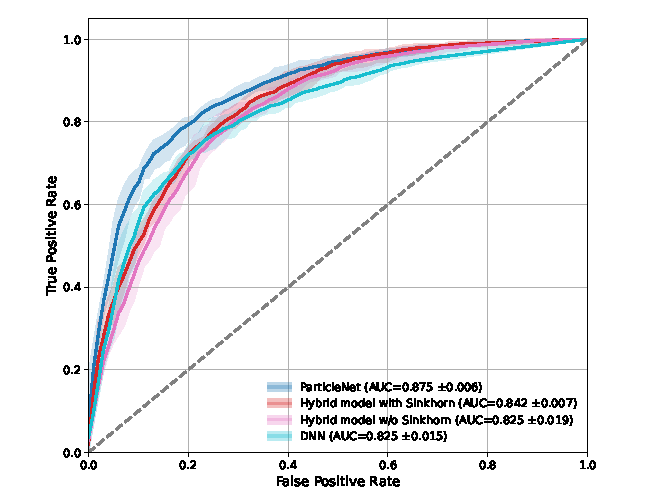
\includegraphics[width=0.7\textwidth]{ch1_roc_final}
\caption{منحنی‌های \lr{ROC} برای آموزش هم‌زمان رمزگذار کلاسیک و \lr{QGNN}، با سینخورن و بدون آن، در مقایسه با یک جداکننده معمولی (\lr{DNN}) و معیار. نوارهای سایه‌دار بازه $\pm1\sigma$ حاصل از اعتبارسنجی متقاطع پنج‌گانه را نشان می‌دهند.}
\label{fig:ch1-roc}
\end{figure}

\begin{table}[H]
\centering
\caption{مقایسه روش‌ها بر حسب توان ردّ پس‌زمینه برای بازدهی‌های شناسایی مختلف جت بوست‌شده.}
\label{tab:ch1-rej}
\begin{tabular}{lccc}
\toprule
بازدهی شناسایی & \lr{25\%} & \lr{60\%} & \lr{80\%} \\
\midrule
\lr{ParticleNet} & $65^{+11}_{-22}$ & $13.0^{+0.4}_{-1.6}$ & $4.8^{+0.1}_{-0.2}$ \\
ترکیبی بدون سینخورن & $26^{+0.4}_{-4}$ & $6.4^{+0.4}_{-0.7}$ & $3.5^{+0.01}_{-0.2}$ \\
ترکیبی با سینخورن & $41^{+23}_{-5}$ & $7.6^{+0.8}_{-0.7}$ & $3.8\pm0.2$ \\
\lr{DNN} & $33^{+7.6}_{-5.5}$ & $8.7^{+1.1}_{-0.2}$ & $3.3^{+0.1}_{-0.15}$ \\
\bottomrule
\end{tabular}
\end{table}
